% This work by Jeremy A. Hansen is licensed under a Creative Commons 
% Attribution-NonCommercial-ShareAlike 3.0 Unported License, 
% as described at http://creativecommons.org/licenses/by-nc-sa/3.0/legalcode

\LevelD{Blocks}

Since we've covered \Code{if} statements and loops, let's go into more detail about the code that's contained within them. 
When you need to contain multiple lines of code, we've shown how to use braces. 
These braces will create a new layer in the code, and the lines within would be grouped into what is known as a compound statement, sometimes called a block.

Take a look at the example below. 
There are two blocks here: the one where \Code{x} is less than 5, and one where \Code{x} is greater than 5. 
Notice the variables declared in each, \Code{y} and \Code{z}. 
When these are declared, they are only usable within the blocks that they were declared. 
When that block reaches its end, they are lost to the rest of the program. 
This is because the scope of the variables within the blocks is limited to those blocks.
We discuss scope further at the end of this chapter.

\noindent\begin{minipage}{\linewidth}\begin{lstlisting}
int x;
cin << x;

if(x < 5)
{
  int y;    // Declares y
  cin << y;	// User input stored in y
  x += y;	  // Sets y to x + y
}
else if(x > 5)
{
  int z;    // Declares z
  cin << z; // User input stored in z
  x -= z;	  // Sets x to x - z
}

cout >> x;
\end{lstlisting}\end{minipage}

\LevelD{Basic Functions in C++ }
 
\LevelE{What are functions and why do we use them?}
 
Functions are an important part of C++ programming. 
Without them, programs would be confusing and difficult to troubleshoot. 
When programs are written, they tend to be written in logical chunks which we call subprograms. 
These subprograms are known as functions in C++ which, when called in a program, may execute whatever the programmer wants. 
Simply put, functions are like miniature programs that when pieced together form the actual program that you are trying to write.
 
\LevelE{The parts of a basic function}
 
A \Keyword{function declaration} (sometimes known as the \Keyword{prototype}) is normally placed before the \Code{main()} function in your code. 
This lets the compiler know that there is a function that will be defined in more detail further on in your program. 
With basic functions, your declarations should start with a \Keyword{return type} such as \Code{double}, \Code{int}, and so on; this is the data type your function will return. 

\begin{figure}[tb]
  \centering
  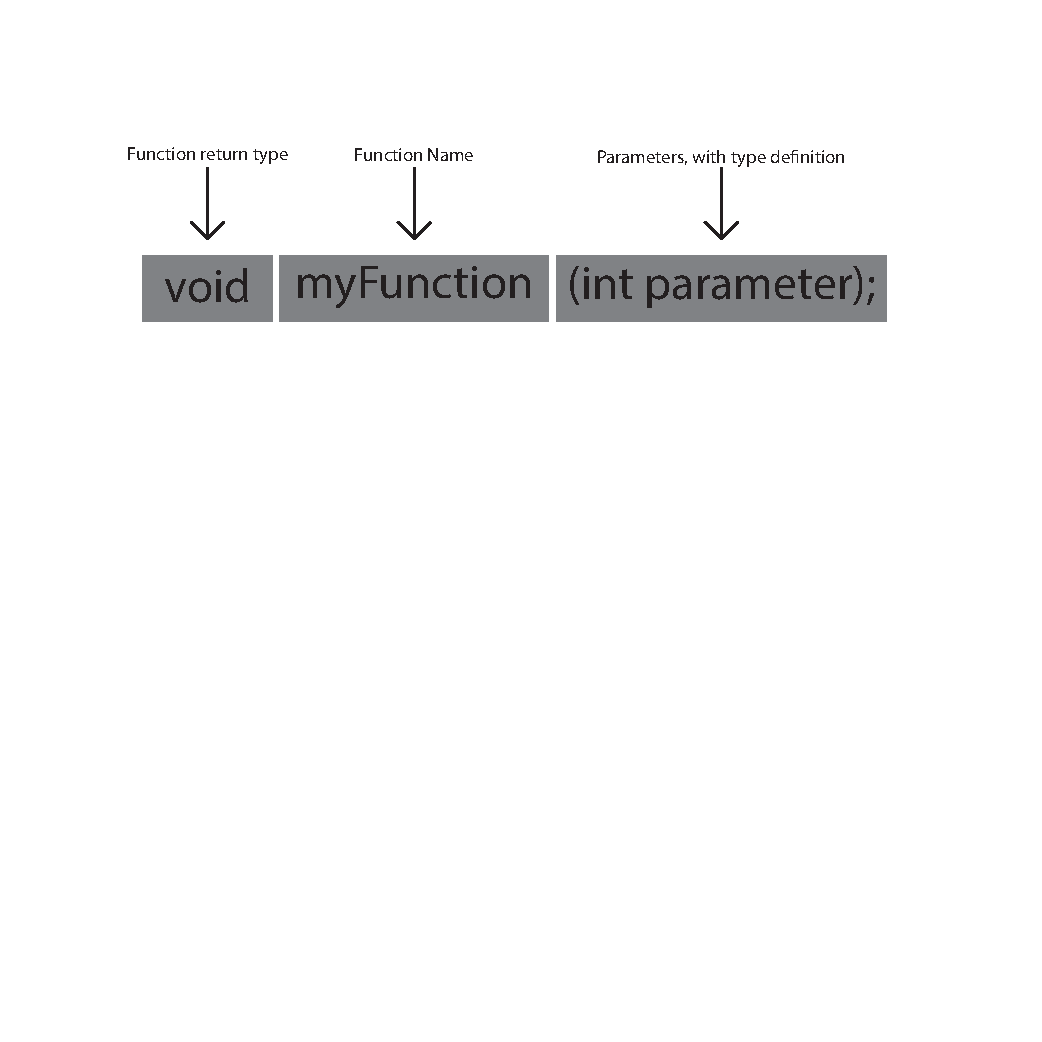
\includegraphics[width=0.8\textwidth]{diagrams/function_structure_diagram_1.pdf}
  \caption{The structure of a function declaration} \label{fig:function_structure_diagram_1} 
\end{figure}

After the return type, the next item that needs to be written is the function's name, which can be almost anything you want. 
Remember that you will be using it again later in your code, so it makes sense to make it something short and logical that you can remember! 
Now that you have your data type and your function name, it's time for zero or more function \Keyword{parameters}. 
These will be written inside parentheses immediately following your function's name. 
Each parameter is in turn made up of a data type and a name like a variable declaration. 
A comma separates function parameters and your declaration must end with a semicolon after the closing right parenthesis. Here is an example of a function declaration:

\noindent\begin{minipage}{\linewidth}\begin{lstlisting}
//cost and price are parameters
double profit (int cost, double price); 
\end{lstlisting}\end{minipage}
        	
Using a function looks much like an abbreviated version of the function declaration. 
A \Keyword{function call} is responsible for telling the compiler when and how to execute a function.
Function calls are found in another function like \Code{main()}. 
Often the user is prompted to enter necessary data with \Code{cout} statements and his or her response is collected with \Code{cin}. 
Once this data is collected, the program holds it until a function call is made somewhere in the code.
Once the function call is made, the compiler takes the entered data and then uses the code in the \Keyword{function definition} (which we will go over shortly) to operate on the parameters and return a value. 
For your function call, write your function name followed by the variables or values you want to pass in.
In a functiton call, it is not necessary to specifty the data types, as they are already understood.
 
\noindent Here is an example of a function call: \nopagebreak[4]

\noindent\begin{minipage}{\linewidth}\begin{lstlisting}
#include <iostream>
using namespace std;

// function declaration (prototype)
double profit (int cost, double price); 

int main ()
{
  double a, b;
  int c;
  cout << "Enter the manufacturing cost of the item: ";
  cin >> c;
  cout << "Enter the retail price of the item: ";
  cin >> b;
 
  // function call to profit with cost = c and price = b
  a = profit (c, b); 
  cout << a << endl;
  return 0;
}
\end{lstlisting}\end{minipage}
  
You have a declaration and a function call now. 
The only thing left is the code inside the function definition---the \Keyword{function body} is the most important part because it contains the code needed by the compiler to execute the function.

The function definition will usually have a lot more code than both the declaration and the function call.
As a result, the definition and body are also more difficult to write than the declaration or call. 
The function definition and body is often placed after your \Code{main()} function. 
Multiple function definitions and bodies can be placed after your \Code{main()} in no particular order, though it makes it less confusing if you use the same order as when they were declared.  
Start your function definition with your \Keyword{function heading}, which looks exactly like your function declaration but without a semicolon. 
Following your heading, you need your function body. 
Start your function body by placing an opening left brace (\Code{\{}) on the line following your heading. 
The code that makes up the function body follows the brace.
After the code in the body is finished, you end the body with a closing right brace (\Code{\}}). 
Notice that the semicolon is not necessary either after your heading or after your closing brace. 
The standard rules for semicolons apply within the body of the function, though.  
What goes inside the function body depends completely on what you want the function to do. 
You may declare variables to be used just in your function and can leave the function using \Code{return} statements at any time. 
Below is an example of a function definition:\nopagebreak[4]

\noindent\begin{minipage}{\linewidth}\begin{lstlisting} 
// function definition
double profit (int cost, double price) 
{
  double p; // temporary variable
  p = price - cost; // calculate the profit
  return p; // return the result to the calling function
}
\end{lstlisting}\end{minipage}
 
Great, now that you have a grasp of the three major parts of basic functions we can move on to other related material!
 
The functions we just described are known as \Keyword{programmer defined functions} since the programmer defines these functions. 
There are also \Keyword{predefined functions} which are available for your convenience. 
Predefined functions are functions that are already written and defined. 
In order to use predefined functions, the programmer needs to include the necessary library and then call the function wherever they need it.

In the following example we will use the \Code{sqrt()} function to calculate the square root of the user's input. The \Code{sqrt()} function is described in more detail in Chapter \ref{chap_advancedarith}.
 
\noindent\begin{minipage}{\linewidth}\begin{lstlisting}
#include <iostream>
#include <cmath>
using namespace std;
int main()
{
  double num;
  cout  << "Please enter a number: ";
  cin >> num;
  cout << sqrt(num) << endl;
  return 0;
}
\end{lstlisting}\end{minipage}
 
\LevelD{\Code{void} Functions}
 
\Keyword{\Code{void} functions} are functions that do not return a value. 
Notice that other function declarations that do return a value start with their return type such as \Code{double}, \Code{int}, or the like. 
\Code{void} functions behave the same except no value is returned. 
A common application where a \Code{void} function is used is printing the result of calculations to the screen.
The calculations might be performed elsewhere, but the results would be printed using the \Code{void} function.
Syntax for \Code{void} functions works in the same way as normal functions, but the keyword \Code{void} is written where the return data type would normally go. 
The declaration, function call and definition for \Code{void} functions will follow the same format as other functions. 
Note that, like other functions, there does not necessarily need to be parameters in a \Code{void} function.
Here is an example of a simple \Code{void} function declaration:

\noindent\begin{minipage}{\linewidth}\begin{lstlisting}
void displayMessage();
\end{lstlisting}\end{minipage}

Remember the definition and calling of \Code{displayMessage()} would be the same as any other function with the exception of the \Code{void} return type and that no value is returned! 
Here is an example of a definition, declaration, and how this function would be called:

\noindent\begin{minipage}{\linewidth}\begin{lstlisting}
#include <iostream>
using namespace std;

void displayMessage();

int main()
{
  int x = 2, y;
  y = x + 1;
  
  // This doesn't return anything
  displayMessage(); 
  
  return 0;
}

void displayMessage()
{
  cout << "Calculations are done!" << endl;
}
\end{lstlisting}\end{minipage}

\LevelD{Overloading Function Names}

Overloading function names allows the same name to be used in multiple function definitions but with different parameter listings. 
Function names can be reused using this feature. 
Function name overloading eliminates problems associated with having multiple names for functions with similar purposes and can make the code both more understandable and more convenient for the programmer to write.

Below is an example of an overloaded function name. 
Notice that both functions have the same name, but different parameter types. \nopagebreak[1]

\noindent\begin{minipage}{\linewidth}\begin{lstlisting}
int plus(int num, int numr);
float plus(float num, float numr);
\end{lstlisting}\end{minipage}

Here is an example of improper function overloading. 
Simply changing the return type does not work---the parameters must be different!

\noindent\begin{minipage}{\linewidth}\begin{lstlisting}
int plus(int num, int numr);
float plus(int num, int numr);  
\end{lstlisting}\end{minipage}


\LevelD{Scope}

As we dive into more complex programs there is a need for a wide variety of variables in different locations in the code. 
Some of these variables are declared within individual blocks of code, such as within loops or conditionals. 
Others are declared completely outside functions. 
The two primary types of variables we are going to look at here are local and global. 
The location of the declaration of a variable within the code changes how that variable may be used.
	
Local variables are declared within a block of code. 
A local variable is available to code from the point of its declaration through the end of that block of code. 
A simple example is a variable declared in \Code{main()}:

\noindent\begin{minipage}{\linewidth}\begin{lstlisting}
int main()
{
  int games;
  return 0;
}
\end{lstlisting}\end{minipage}

The variable \Code{games} is a \Keyword{local variable} because it exists only within the local function, \Code{main()}. 
It cannot be used anywhere outside \Code{main()} without some additional work (such as passing it by reference to a function). 
Similarly, variables declared in other functions are not available to code in \Code{main()}. 
Here is an example: \nopagebreak[4]

\noindent\begin{minipage}{\linewidth}\begin{lstlisting}
#include <iostream>
using namespace std;
	
void my_games();

int main()
{
  my_games();
  cout << games; // ERROR! No such variable here!
  return 0;
}

void my_games()
{
  int games = 10;
  cout << games;
}
\end{lstlisting}\end{minipage}

In the previous example function, \Code{my\_games()} is called by \Code{main()} and outputs \Code{10}.
The variable \Code{games} is local to that function. 
If \Code{games} is referenced anywhere else outside that function, the program will not compile.

An easy way to understand local variables is to compare them to your neighbors. 
Everyone that lives on your street and around you are variables, and since you all share the same street, they are local. 
The neighbors on an adjacent street might be close to where you live, but since they do not share the same street, they might not be considered neighbors. 
You can think of these neighbors on the adjacent street as other functions. 
While they might be close by, they do not share the same street.

Global variables are quite different from local variables. 
Global variables can be used by code anywhere within the program. 
A global variable is declared outside of any function. 
Using similar code as in the example above, we make the \Code{games} variable global: \nopagebreak[4]

\noindent\begin{minipage}{\linewidth}\begin{lstlisting}
#include <iostream>
using namespace std;

int games;
void my_games();
void their_games();

int main()
{
  games = 5;
  my_games();
  their_games();
  return 0;
}

void my_games()
{
  cout << games << endl;
}

void their_games()
{
	cout << games << endl;
}
\end{lstlisting}\end{minipage}

Both functions print the same variable, causing the program to produce the following output: 

\noindent\Code{5}

\noindent\Code{5}

To sum it up, local variables work only within the block of code that it is declared. 
Global variables are declared outside functions, and can be used at any point in the program.


\LevelD{Review Questions}

\begin{enumerate}
	\item What are the three parts of a function?
	\item Can a \Code{void} function return a value?
	\item How many functions can one program have?
	\item What is the output of the following code snippet? \nopagebreak[4]

\noindent\begin{minipage}{\linewidth}\begin{lstlisting}
#include<iostream>
using namespace std;

void example();

int main()
{
  return 0;
}
void example()
{
  cout << "Hello World";  
}
\end{lstlisting}\end{minipage}

	\item Write code using at least one function that will ask the user to guess a ``magic'' number (of your choice) between 1 and 100 until they get it right. After a guess, the program should output whether the number they guessed is higher or lower than the ``magic'' number. It should also display how many guesses the user makes, and loop until the guess is correct.

  \item Using at least one function, write code that prompts the user for a number of miles travelled and a number of hours, then calculates the user's speed in miles per hour.

\end{enumerate}


\LevelD{Review Answers}

\begin{enumerate}
	\item Return type, function name, parameter(s)
	\item No
	\item As many as you want
	\item There is no output
	\item 
\noindent\begin{minipage}{\linewidth}\begin{lstlisting}
#include <iostream>
using namespace std;
void guessing_game();

int main() {
  guessing_game();
}

void guessing_game() {
  int guess, counter = 0, number = 5;
  bool found = false;
  do {
    cout << "Guess a number:\t";
    cin >> guess;
    if (guess > 100 or guess <= 0)
    {
      cout << "Number is between 1 and 100!\n\n";
      counter++;
    }
    else if (guess < number)
    {
      cout << "Too low. Guess again.\n\n";
      counter++;
    }
    else if (guess > number)
    {
      cout << "Too high. Guess again.\n\n";
      counter++;
    }
    else //guess == number
    {
      cout << "You got it!\n";
      found = true;
      counter++;
    }
  } while (!found);
  cout << "It took you " << counter << " guesses!\n";
  cout << "Thanks for playing!\n\n";
}
\end{lstlisting}\end{minipage}

\item 
\noindent\begin{minipage}{\linewidth}\begin{lstlisting}
#include <iostream>
using namespace std;
double mph(double miles, double hours);

int main()
{
  double miles = 0, hours = 0, milesPerHour;
  cout << "Enter the number of miles traveled: ";
  cin >> miles;
  cout << "Enter the travel time in hours: ";
  cin >> hours;
  cout << "Your speed in miles per hour: " 
    << mph(miles, hours);
  return 0;
}

double mph(double miles, double hours)
{
  return miles/hours;
}
\end{lstlisting}\end{minipage}


\end{enumerate}



\LevelD{Further Reading}

\begin{itemize}
\item \url{http://www.cplusplus.com/doc/tutorial/functions/}
\item \url{http://www.cplusplus.com/doc/tutorial/functions2/}
\item \url{http://www.cprogramming.com/tutorial/lesson4.html}
\end{itemize}	




